%~ Questo sorgente è stato scritto da Giovan Battista Rolandi
%~ è rilasciato sotto licenza GPL3
%~ ed è consultabile presso
%~ http://golem.linux.it/ (HTTP)
%~ git@github.com:giomba/beamer-intro-linux.git (GIT/SSH)

% \documentclass[handout]{beamer} %% stile di stampa su carta

\documentclass{beamer}
\usepackage[italian]{babel}
\usepackage[utf8]{inputenc}
\usepackage[font=scriptsize]{caption}
\usepackage{fancyvrb}

\usetheme{Madrid}
\colorlet{beamer@blendedblue}{green!40!black}
%~ \usetheme{Luebeck}
%~ \usetheme{Berkeley}
%~ \usetheme{Goettingen}
%~ \usetheme{Rochester}
%~ \usetheme{Singapore}
\setbeamertemplate{caption}[numbered]
\setbeamercovered{dynamic}

\beamertemplatenavigationsymbolsempty

\title{Introduzione al software libero}
%\subtitle{}
\logo{
\includegraphics[width=5em]{img/logo-linuxday.pdf}}
\author{giomba}
\date{28 ottobre 2017}
\institute{GOLEM Empoli}

\begin{document}

\begin{frame}
  \maketitle
  \tableofcontents
\end{frame}

\begin{frame}[fragile]
\frametitle{Un po' di storia}

    \begin{block}{Anni 1960}
	\begin{minipage}{.15\linewidth}
	    
\includegraphics[width=.9\linewidth]{img/meeting.png}
	\end{minipage}
    \begin{minipage}{.8\linewidth}
    I programmatori di computer sono soliti condividere il proprio lavoro
    \begin{exampleblock}{Codice}
    \begin{minipage}{.45\linewidth}
        \begin{Verbatim}[fontsize=\scriptsize]
int main() {
    int risultato = 1,
    base = 2,
    esponente = 4;
    for (int i = 0;
    i < esponente;
    ++i) {
    risultato *= base;
    }
}
        \end{Verbatim}
    \end{minipage}
    \begin{minipage}{.45\linewidth}
        \begin{Verbatim}[fontsize=\scriptsize]
55
48 89 e5
c7 45 f0 01 00 00 00
[...]
8b 45 f4
3b 45 fc
7d 10
8b 45 f0
0f af 45 f8
89 45 f0
83 45 f4 01
eb e8
b8 00 00 00 00
5d
c3
        \end{Verbatim}
    \end{minipage}
    \end{exampleblock}
    \end{minipage}
    \end{block}
\end{frame}

\begin{frame}
\frametitle{Chiusura del software}

    \begin{block}{Anni 1970}
    \begin{itemize}
        \item
        \begin{minipage}{.2\linewidth}
            
\includegraphics[width=.9\linewidth]{img/lock.png}
        \end{minipage}
        \begin{minipage}{.7\linewidth}
            Interessi commerciali impongono la nascita di "accordi di non-divulgazione"
        \end{minipage}
        \pause
        \item
        \begin{minipage}{.2\linewidth}
            \visible<2->{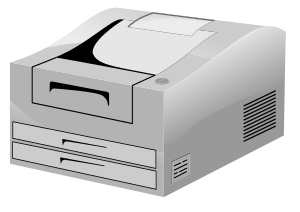
\includegraphics[width=.9\linewidth]{img/laserprinter.png}}
        \end{minipage}
        \begin{minipage}{.7\linewidth}
            La Xerox regala una nuova stampante laser dal software chiuso all'IA~Lab del MIT
        \end{minipage}
    \end{itemize}
    \end{block}
\end{frame}


\begin{frame}
    \frametitle{Richard Stallman, il free software e GNU}

    \begin{minipage}{.4\linewidth}
    \begin{figure}
    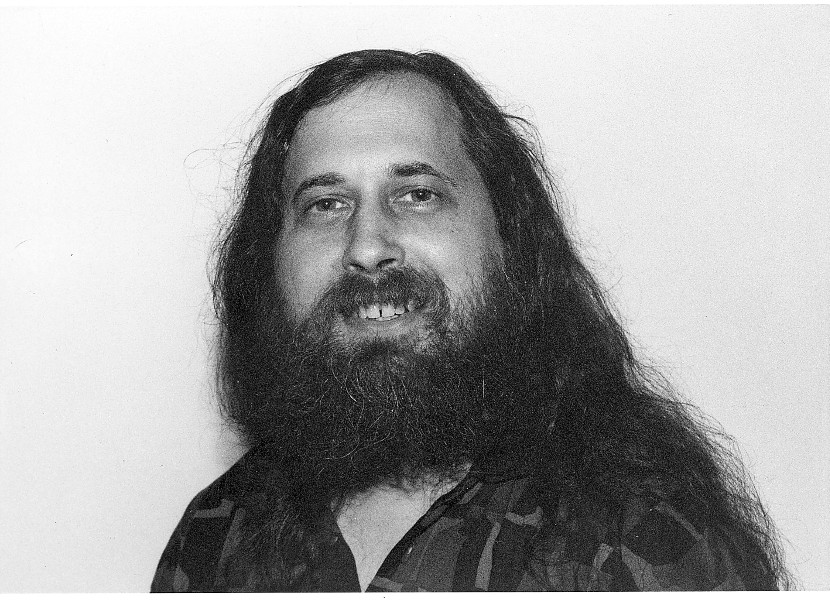
\includegraphics[width=.9\linewidth]{img/rms.jpeg}
    \caption{Richard~Matthew Stallman}
    \end{figure}
    \end{minipage}
    \pause
    \begin{minipage}{.55\linewidth}
    \begin{block}{Software libero}
        \begin{enumerate}
        \setcounter{enumi}{-1}
        \item libertà di poter utilizzare il programma per qualunque scopo
        \item libertà di poter studiare il funzionamento del programma
        \item libertà di poter modificare il programma
        \item libertà di poter ridistribuire il programma modificato
        \end{enumerate}
    \end{block}
    \pause
    \begin{block}{1984}
        \begin{minipage}{.2\linewidth}
        \visible<3->{
\includegraphics[width=1\linewidth]{img/gnu.pdf}}
        \end{minipage}
        \begin{minipage}{.75\linewidth}
        Nasce GNU, sistema operativo completamente libero basato su Unix
        \end{minipage}
    \end{block}
    \end{minipage}
\end{frame}

\begin{frame}
    \frametitle{Linus Torvalds e Linux}

    \begin{minipage}{.4\linewidth}
    \begin{figure}
        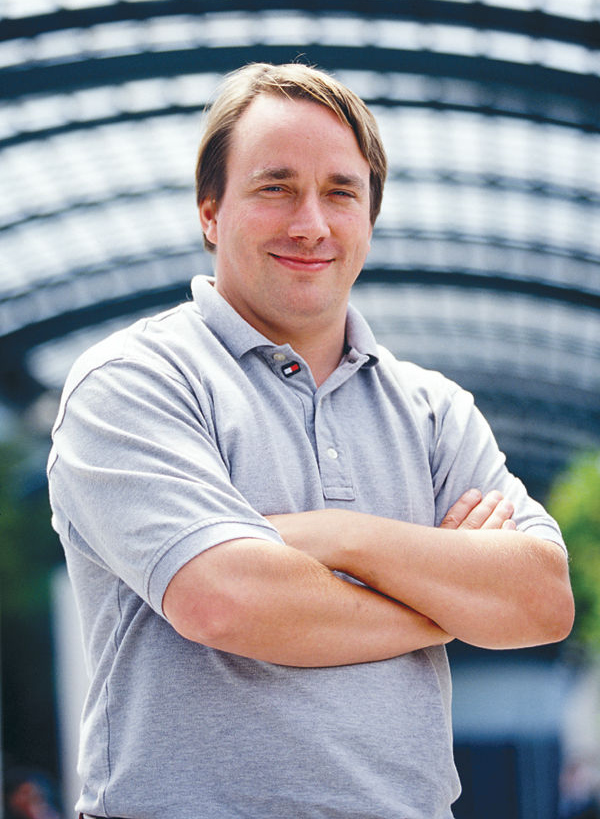
\includegraphics[width=.9\linewidth]{img/torvalds.jpeg}
        \caption{Linus Benedict Torvalds}
        \end{figure}
    \end{minipage}
    \begin{minipage}{.55\linewidth}
        \begin{block}{Perché}
            \begin{itemize}
                \item
                    \begin{minipage}{.2\linewidth} \visible<1->{
\includegraphics[width=.9\linewidth]{img/i-3-unix.pdf}} \end{minipage}
                    \begin{minipage}{.75\linewidth} All'Università si appassiona ai sistemi Unix \end{minipage}
                    \pause
                \item
                    \begin{minipage}{.2\linewidth} \visible<2->{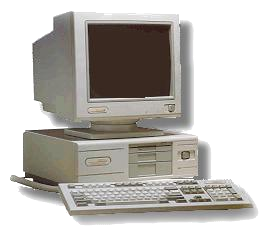
\includegraphics[width=.9\linewidth]{img/pc-i386.png}} \end{minipage}
                    \begin{minipage}{.75\linewidth} Compra un PC i386 a rate \end{minipage}
                    \pause
                \item
                    \begin{minipage}{.2\linewidth} \visible<3->{
\includegraphics[width=.9\linewidth]{img/minix.pdf}} \end{minipage}
                    \begin{minipage}{.75\linewidth} Installa Minix-Unix sul PC \end{minipage}
                    \pause
                \item
                    \begin{minipage}{.2\linewidth} \visible<4->{
\includegraphics[width=.9\linewidth]{img/error.pdf}} \end{minipage}
                    \begin{minipage}{.75\linewidth} Impossibilità di modificare liberamente Minix \end{minipage}
                    \pause
            \end{itemize}
        \end{block}
    \begin{block}{1991}
        \begin{minipage}{.2\linewidth}
        \visible<5->{
\includegraphics[width=1\linewidth]{img/tux.pdf}}
        \end{minipage}
        \begin{minipage}{.75\linewidth}
        Nasce il kernel Linux
        \end{minipage}
    \end{block}
    \end{minipage}
\end{frame}

%~ \begin{frame}
    %~ \frametitle{Lo sviluppo di GNU/Linux}

    %~ \begin{itemize}
        %~ \item 1984 -- Nasce il sistema operativo GNU
        %~ \item 1991 -- Nasce il kernel Linux
        %~ \item 1992 -- Il kernel Linux viene rilasciato sotto licenza GPL
        %~ \item 1993 -- Nascono Slackware e Debian
        %~ \item 1994 -- Nascono Suse e RedHat
        %~ \item 2004 -- Nasce Ubuntu
        %~ \item 2006 -- Nasce Linux Mint
    %~ \end{itemize}
%~ \end{frame}

\begin{frame}
    \frametitle{Le ragioni del successo}

    \begin{itemize}
        \item
            \begin{minipage}{.15\linewidth} \visible<1->{
\includegraphics[width=.9\linewidth]{img/no-cost.pdf}} \end{minipage}
            \begin{minipage}{.8\linewidth} Costo nullo del prodotto \end{minipage}
            \pause
        \item
            \begin{minipage}{.15\linewidth} \visible<2->{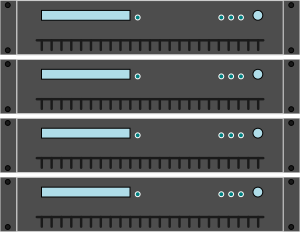
\includegraphics[width=.9\linewidth]{img/servers.png}} \end{minipage}
            \begin{minipage}{.8\linewidth} Supporto multiprocessore e multipiattaforma \end{minipage}
            \pause
        \item
            \begin{minipage}{.15\linewidth} \visible<3->{
\includegraphics[width=.9\linewidth]{img/apache.png}} \end{minipage}
            \begin{minipage}{.8\linewidth} Server web Apache \end{minipage}
            \pause
        \item
            \begin{minipage}{.15\linewidth} \visible<4->{
\includegraphics[width=.9\linewidth]{img/redhat.png}} \end{minipage}
            \begin{minipage}{.8\linewidth} Prodotti commerciali con hardware certificato \end{minipage}
    \end{itemize}
\end{frame}

\begin{frame}
    \frametitle{Potenzialità}

    \begin{columns}
    \begin{column}{.25\textwidth}
        
\includegraphics[width=.9\linewidth]{img/knoppix.png}
        \centering
        Sistemi Live
    \end{column}

    \begin{column}{.25\textwidth}
        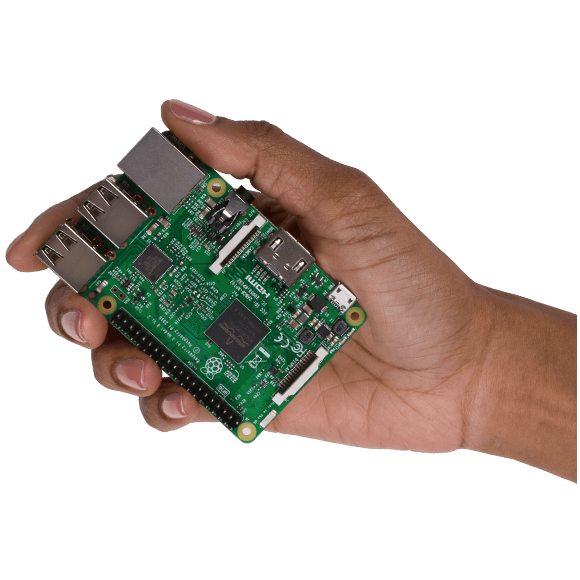
\includegraphics[width=.9\linewidth]{img/raspberry.png}
        \centering
        Minicomputer
    \end{column}

    \begin{column}{.25\textwidth}
        
\includegraphics[width=.9\linewidth]{img/android.png}
        \centering
        Smartphone
    \end{column}

    \begin{column}{.25\textwidth}
        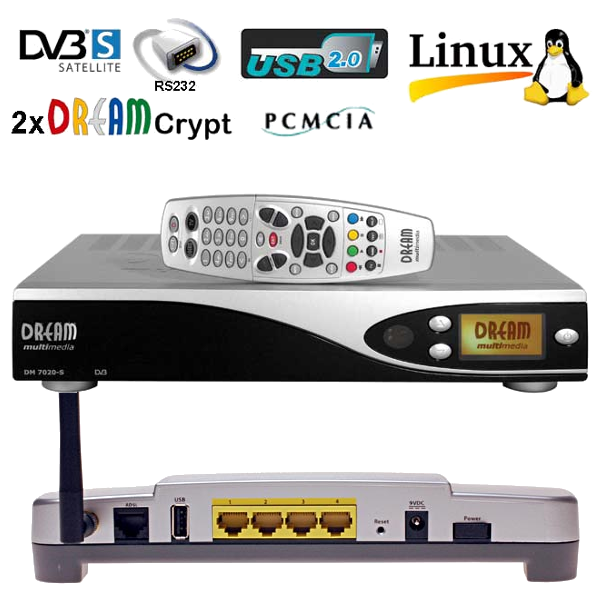
\includegraphics[width=.9\linewidth]{img/router-decoder.png}
        \centering
        Modem, Router
    \end{column}
    \end{columns}

\end{frame}

\begin{frame}
    \frametitle{Le Distribuzioni}

    \begin{minipage}[b][.35\textheight][t]{.3\textwidth}
    
\includegraphics[width=.45\textwidth]{img/gnu.pdf}
    
\includegraphics[width=.45\textwidth]{img/tux.pdf}\\
    \centering
    GNU/Linux
    \end{minipage}\hfill
    \begin{minipage}[b][.35\textheight][t]{.3\textwidth}
    
\includegraphics[width=.7\textwidth]{img/firefox.pdf}\\
    \centering
    Browser
    \end{minipage}\hfill
    \begin{minipage}[b][.35\textheight][t]{.3\textwidth}
    
\includegraphics[width=.7\textwidth]{img/libreoffice.png}\\
    \centering
    Suite Ufficio
    \end{minipage}\\[0.5em]

    \begin{minipage}[b][.35\textheight][t]{.3\textwidth}
    
\includegraphics[width=.7\textwidth]{img/oss.png}\\
    \centering
    Utilità
    \end{minipage}\hfill
    \begin{minipage}[b][.35\textheight][t]{.3\textwidth}
    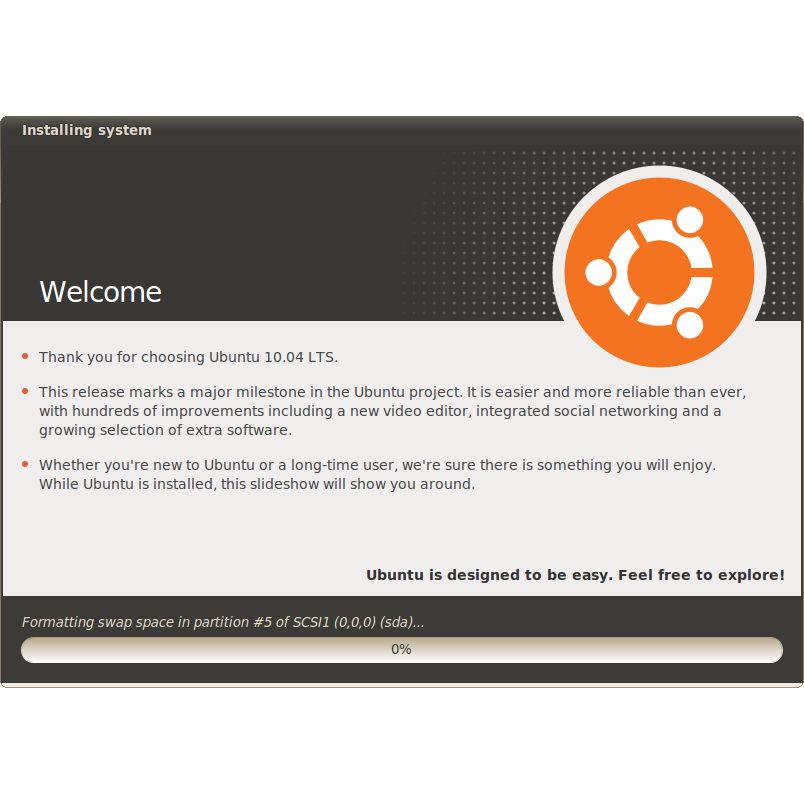
\includegraphics[width=.7\textwidth]{img/ubiquity.png}\\
    \centering
    Installer
    \end{minipage}\hfill
    \begin{minipage}[b][.35\textheight][t]{.3\textwidth}
    
\includegraphics[width=.7\textwidth]{img/mint-dvd.png}\\
    \centering
    Distribuzione
    \end{minipage}
\end{frame}

\begin{frame}
    \frametitle{Le distribuzioni più famose}

    \begin{minipage}[b][.35\textheight][t]{.3\textwidth}
    
\includegraphics[width=.7\textwidth]{img/logo-debian.pdf}\\
    \end{minipage}\hfill
    \begin{minipage}[b][.35\textheight][t]{.3\textwidth}
    
\includegraphics[width=.7\textwidth]{img/logo-ubuntu.png}\\
    \centering
    Ubuntu
    \end{minipage}\hfill
    \begin{minipage}[b][.35\textheight][t]{.3\textwidth}
    
\includegraphics[width=.7\textwidth]{img/logo-linuxmint.pdf}\\
    \centering
    LinuxMint
    \end{minipage}\\[0.5em]

    \begin{minipage}[b][.35\textheight][t]{.3\textwidth}
    
\includegraphics[width=.7\textwidth]{img/logo-fedora.pdf}\\
    \centering
    Fedora
    \end{minipage}\hfill
    \begin{minipage}[b][.35\textheight][t]{.3\textwidth}
    
\includegraphics[width=.7\textwidth]{img/logo-centos.pdf}\\
    \end{minipage}\hfill
    \begin{minipage}[b][.35\textheight][t]{.3\textwidth}
    
\includegraphics[width=.7\textwidth]{img/redhat.png}\\
    \centering
    RHEL
    \end{minipage}

\end{frame}

\begin{frame}
    \frametitle{Tutte le distribuzioni}

    \includegraphics[width=1\linewidth]{img/linux-distribution-timeline.pdf}
    \centering
    Linux Distribution Timeline
\end{frame}

\begin{frame}
    \frametitle{Comunità}

    \begin{block}{anni 1990}
    \begin{itemize}
        \item Nascono i LUG -- Linux Users Group
        \item 1994 -- Nasce la Italian Linux Society
        \item 2000 -- Nasce il GOLEM
    \end{itemize}
    \end{block}
    \pause

    \begin{block}{GOLEM - Gruppo Operativo Linux Empoli}
        \begin{minipage}{.1\linewidth}
            \visible<2->{
\includegraphics[width=1\linewidth]{img/GOLEM-logo.pdf}}
        \end{minipage}
        \begin{minipage}{.55\linewidth}
            \begin{itemize} % [<+->]
                \item Ore del GOLEM
                \item Arduino Project Day
                \item Trashware
                \item Corsi, campagne di sensibilizzazione, eventi promozionali, Linux Day
            \end{itemize}
        \end{minipage}
        \begin{minipage}{.3\linewidth}
            \visible<2->{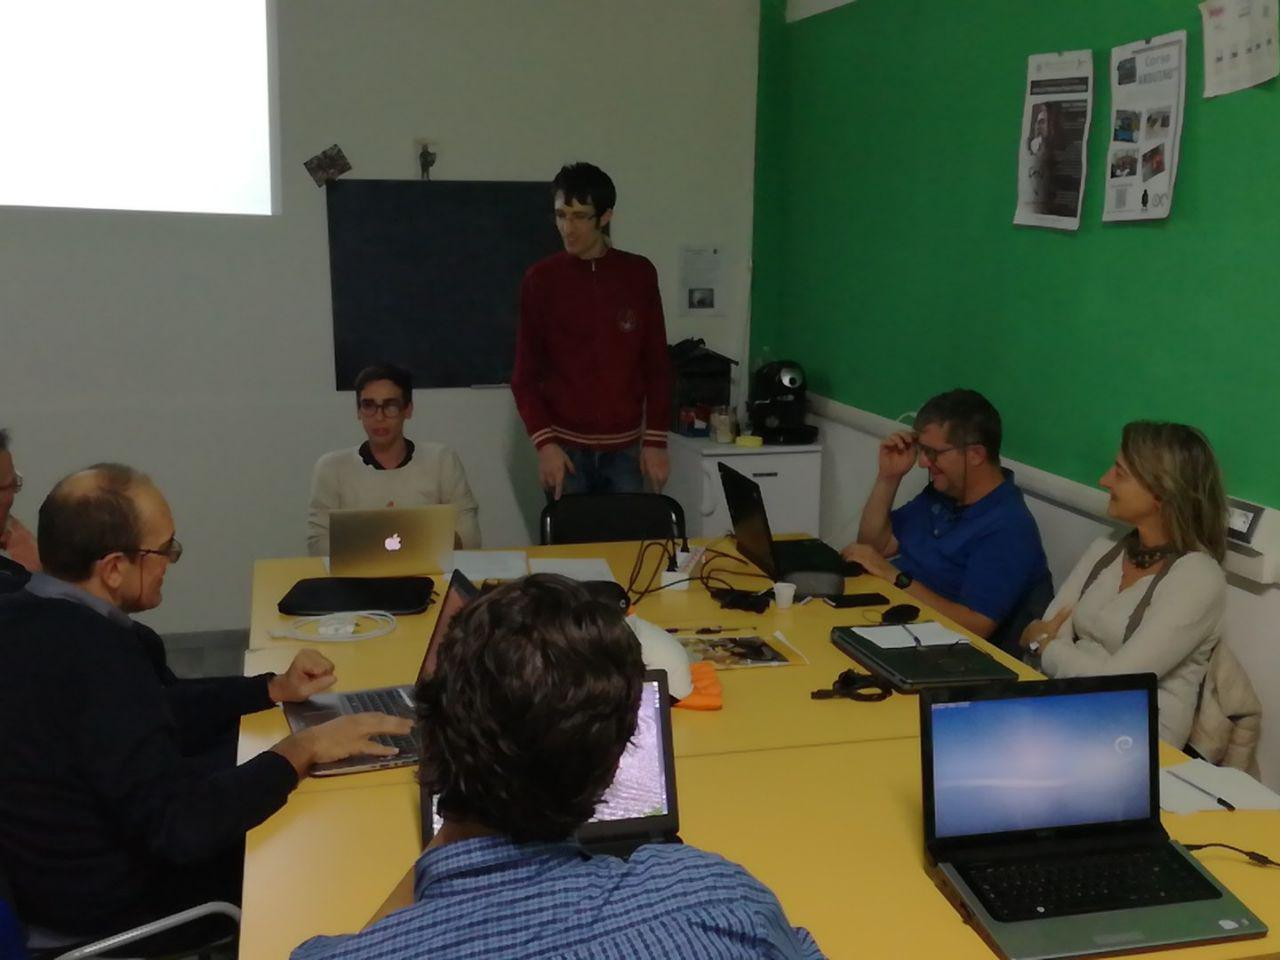
\includegraphics[width=1\linewidth]{img/GOLEM-foto.jpeg}}
        \end{minipage}
    \end{block}
\end{frame}

\begin{frame}
  \frametitle{Introduzione al software libero}

    \begin{block}{GOLEM - Gruppo Operativo Linux Empoli}
        \begin{minipage}{.15\linewidth}
            
\includegraphics[width=1\linewidth]{img/GOLEM-logo.pdf}
        \end{minipage}
        \begin{minipage}{.65\linewidth}
            \centering
            GOLEM -- Gruppo Operativo Linux Empoli\\
            presso "La Vela -- Margherita Hack"\\
            via Magolo, 32 -- 50053 Empoli (FI)\\
            tutti i martedì sera dalle 21.30 alle 24.00
        \end{minipage}
        \begin{minipage}{.15\linewidth}
            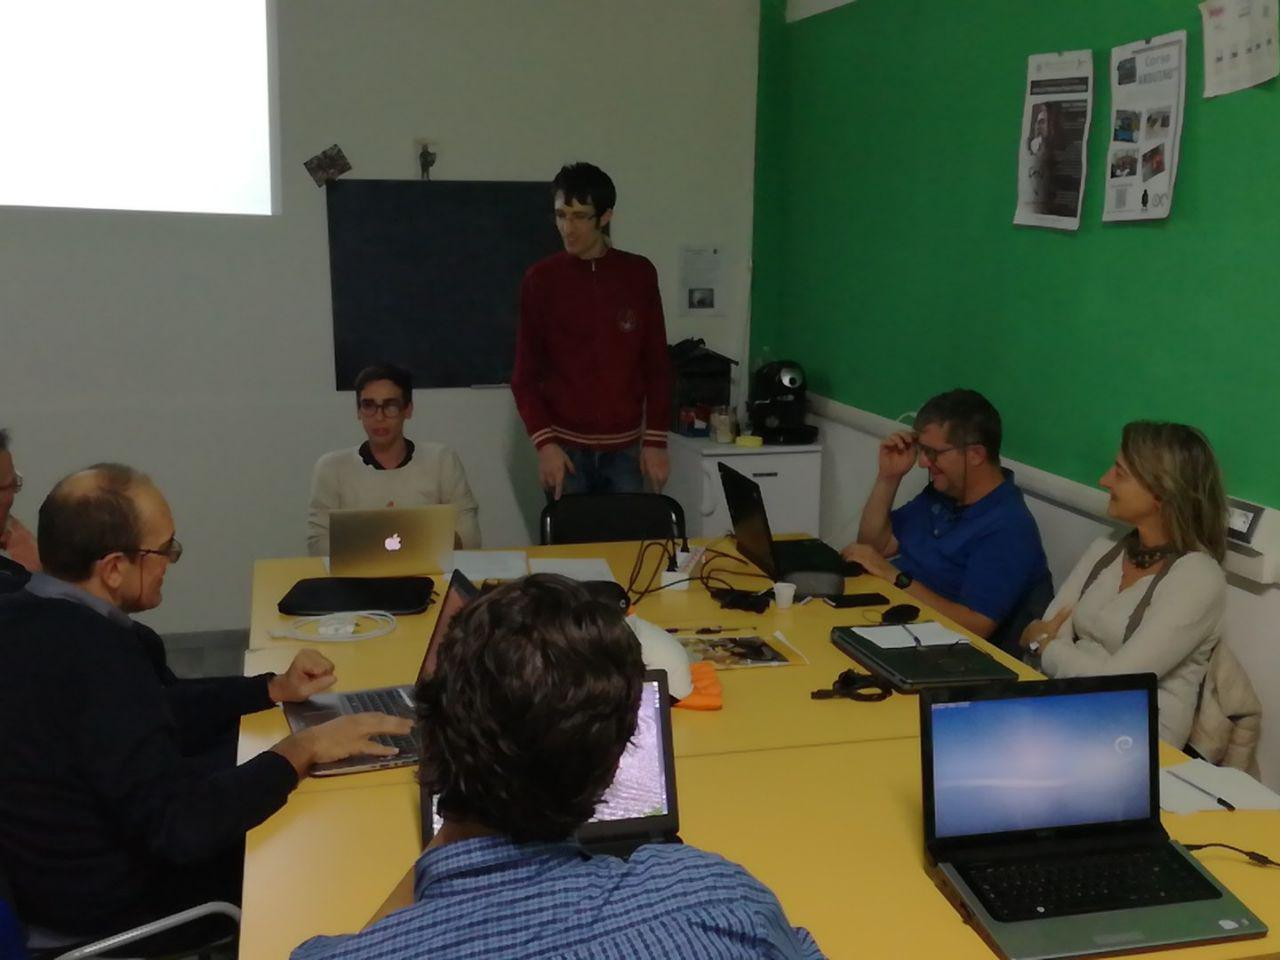
\includegraphics[width=1\linewidth]{img/GOLEM-foto.jpeg}
        \end{minipage}
    \end{block}

    \begin{block}{Linux Day}
    \centering
    \begin{minipage}{.15\linewidth}
      
\includegraphics[width=1\linewidth]{img/linuxday-logo.png}
    \end{minipage}
    \begin{minipage}{.65\linewidth}
    \centering
    Questa presentazione è stata preparata\\ % da\\
    %~ GOLEM -- Gruppo Operativo Linux Empoli\\
    in occasione del Linux Day 2017\\
    e viene rilasciata sotto GPL3\\
    presso golem.linux.it\\
    \copyright Giovan Battista Rolandi (giomba)\\
    giomba@linux.it -- GPG: 5F94294D
    \end{minipage}
    \begin{minipage}{.15\linewidth}
      
\includegraphics[width=1\linewidth]{img/gpl3.pdf}
    \end{minipage}
    \end{block}

  %~ \begin{block}{Licenza}
    %~ \centering
    %~ \begin{minipage}{.18\linewidth}
      %~ \begin{figure}
        %~ \centering
        %~ 
\includegraphics[width=.9\linewidth]{img/gnu.pdf}
      %~ \end{figure}
    %~ \end{minipage}
    %~ \hfill
    %~ \begin{minipage}{.6\linewidth}
      %~ \centering
      %~ Il sorgente di questa presentazione\\
      %~ è software libero,\\
      %~ viene rilasciato sotto licenza GPLv3,\\
      %~ ed è consultabile presso golem.linux.it
    %~ \end{minipage}
    %~ \hfill
    %~ \begin{minipage}{.18\linewidth}
      %~ \begin{figure}
        %~ \centering
        %~ 
\includegraphics[width=.9\linewidth]{img/gpl3.pdf}
      %~ \end{figure}
    %~ \end{minipage}

  %~ \end{block}

\end{frame}

\end{document}
